\PassOptionsToPackage{unicode}{hyperref}
\PassOptionsToPackage{hyphens}{url}
\PassOptionsToPackage{dvipsnames,svgnames,x11names}{xcolor}
\documentclass[
  spanish,
  11pt,
  a4paper,
  DIV=11,
  numbers=noendperiod]{scrartcl}

\usepackage{xcolor}
\usepackage[top=24mm,bottom=24mm,left=24mm,right=24mm,headheight=15pt,headsep=8mm]{geometry}
\usepackage{amsmath,amssymb}
\usepackage{iftex}
\ifPDFTeX
  \usepackage[T1]{fontenc}
  \usepackage[utf8]{inputenc}
  \usepackage{textcomp}
\else
  \usepackage{unicode-math}
  \defaultfontfeatures{Scale=MatchLowercase}
  \defaultfontfeatures[\rmfamily]{Ligatures=TeX,Scale=1}
\fi
\usepackage{lmodern}
\IfFileExists{upquote.sty}{\usepackage{upquote}}{}
\IfFileExists{microtype.sty}{
  \usepackage[]{microtype}
  \UseMicrotypeSet[protrusion]{basicmath}
}{}
\usepackage{graphicx}
\usepackage{float}
\usepackage[bidi=basic]{babel}
\let\LanguageShortHands\languageshorthands
\def\languageshorthands#1{}
\setlength{\emergencystretch}{3em}
\setcounter{secnumdepth}{5}
\providecommand{\tightlist}{\setlength{\itemsep}{0pt}\setlength{\parskip}{0pt}}

\newcommand{\practicaPdfCoverImage}{../resources/practica7/images/teaser_horizontal.jpg}
% PDF style for Practica 9.
% A modest university handout look: classical type, clear hierarchy,
% restrained color, and durable code/callout styling.

\usepackage{graphicx}
\usepackage[export]{adjustbox}
\usepackage{fontspec}
\usepackage{microtype}
\usepackage{scrlayer-scrpage}
\usepackage{tikz}
\usepackage{fvextra}
\usepackage{caption}
\usepackage{subcaption}
\usepackage[skins,breakable]{tcolorbox}

\providecommand{\practicaPdfCoverImage}{}

\definecolor{uzaInk}{HTML}{172033}
\definecolor{uzaMuted}{HTML}{5F6B7A}
\definecolor{uzaBlue}{HTML}{1F5F8B}
\definecolor{uzaBlueDark}{HTML}{153E5C}
\definecolor{uzaCyan}{HTML}{EAF4F7}
\definecolor{uzaLine}{HTML}{D7E2EA}
\definecolor{uzaCodeBg}{HTML}{F5F7F9}
\definecolor{uzaTip}{HTML}{237A57}
\definecolor{uzaWarn}{HTML}{A65F00}

\IfFontExistsTF{TeX Gyre Pagella}{
  \setmainfont{TeX Gyre Pagella}
}{}
\IfFontExistsTF{TeX Gyre Heros}{
  \setsansfont{TeX Gyre Heros}
}{}
\IfFontExistsTF{TeX Gyre Cursor}{
  \setmonofont{TeX Gyre Cursor}[Scale=0.86]
}{
  \setmonofont{Latin Modern Mono}[Scale=0.88]
}

\KOMAoptions{parskip=half}
\setlength{\parindent}{0pt}
\setlength{\parskip}{0.55em plus 0.15em minus 0.08em}
\linespread{1.035}

\addtokomafont{disposition}{\sffamily\color{uzaBlueDark}}
\addtokomafont{section}{\LARGE}
\addtokomafont{subsection}{\Large}
\addtokomafont{subsubsection}{\normalsize\bfseries}
\RedeclareSectionCommand[beforeskip=2.2em plus 0.4em minus 0.2em,afterskip=1.0em]{section}
\RedeclareSectionCommand[beforeskip=1.2em,afterskip=0.55em]{subsection}
\RedeclareSectionCommand[beforeskip=1.0em,afterskip=0.35em]{subsubsection}

\clearpairofpagestyles
\automark[section]{section}
\ihead{\sffamily\footnotesize\textcolor{uzaMuted}{Informática (30717)}}
\ohead{\sffamily\footnotesize\textcolor{uzaMuted}{\headmark}}
\cfoot{\sffamily\small\textcolor{uzaMuted}{\pagemark}}
\setkomafont{pageheadfoot}{\normalfont}
\KOMAoptions{headsepline=0.35pt}
\addtokomafont{headsepline}{\color{uzaLine}}

\makeatletter
\AtBeginDocument{%
  \hypersetup{
    linkcolor=uzaBlueDark,
    urlcolor=uzaBlue,
    citecolor=uzaBlueDark
  }%
  \@ifundefined{Highlighting}{%
    \DefineVerbatimEnvironment{Highlighting}{Verbatim}{
      commandchars=\\\{\},
      fontsize=\small,
      breaklines=true,
      breakanywhere=true
    }%
  }{%
    \RecustomVerbatimEnvironment{Highlighting}{Verbatim}{
      commandchars=\\\{\},
      fontsize=\small,
      breaklines=true,
      breakanywhere=true
    }%
  }%
  \@ifundefined{Shaded}{%
    \newenvironment{Shaded}{%
      \begin{tcolorbox}[
        enhanced,
        breakable,
        sharp corners,
        boxrule=0.25pt,
        colback=uzaCodeBg,
        colframe=uzaLine,
        borderline west={1.4pt}{0pt}{uzaBlue},
        left=2mm,
        right=2mm,
        top=1.4mm,
        bottom=1.4mm,
        before skip=0.75em,
        after skip=0.75em
      ]%
    }{%
      \end{tcolorbox}%
    }%
  }{%
    \renewenvironment{Shaded}{%
      \begin{tcolorbox}[
        enhanced,
        breakable,
        sharp corners,
        boxrule=0.25pt,
        colback=uzaCodeBg,
        colframe=uzaLine,
        borderline west={1.4pt}{0pt}{uzaBlue},
        left=2mm,
        right=2mm,
        top=1.4mm,
        bottom=1.4mm,
        before skip=0.75em,
        after skip=0.75em
      ]%
    }{%
      \end{tcolorbox}%
    }%
  }%
}
\makeatother

\newcommand{\PracticeCode}[1]{%
  \begin{Shaded}%
  \VerbatimInput[
    fontsize=\small,
    breaklines=true,
    breakanywhere=true
  ]{#1}%
  \end{Shaded}%
}

\makeatletter
\renewcommand{\maketitle}{%
  \begin{titlepage}
    \thispagestyle{empty}
    \begin{tikzpicture}[remember picture,overlay]
      \fill[uzaCyan] (current page.north west) rectangle ([yshift=-72mm]current page.north east);
      \fill[uzaBlue] (current page.north west) rectangle ([xshift=7mm]current page.south west);
    \end{tikzpicture}
    \vspace*{12mm}
    {\sffamily\small\bfseries\textcolor{uzaBlue}{INFORMÁTICA (30717)}}\par
    \vspace{5mm}
    {\sffamily\bfseries\fontsize{30}{35}\selectfont\textcolor{uzaInk}{\@title}}\par
    \vspace{3mm}
    {\sffamily\Large\textcolor{uzaMuted}{Grado en Estudios en Arquitectura}}\par
    \vspace{8mm}
    {\color{uzaBlue}\rule{\textwidth}{0.6pt}}\par
    \if\relax\detokenize\expandafter{\practicaPdfCoverImage}\relax
    \else
      \vspace{5mm}
      {\centering\includegraphics[width=\textwidth,height=78mm,keepaspectratio]{\practicaPdfCoverImage}\par}
    \fi
    \vfill
    {\sffamily\large\textcolor{uzaBlueDark}{Universidad de Zaragoza}}\par
    \vspace{2mm}
    {\sffamily\small\textcolor{uzaMuted}{Material de prácticas del curso 2025--2026}}\par
  \end{titlepage}
}
\makeatother

\captionsetup{
  font={small,sf},
  labelfont={bf,color=uzaBlueDark},
  textfont={color=uzaInk},
  justification=centering,
  singlelinecheck=false,
  skip=6pt
}
\captionsetup[subfigure]{
  font={small,sf},
  labelfont={bf,color=uzaBlueDark},
  justification=centering,
  singlelinecheck=true,
  skip=4pt
}

\newcommand{\PracticeCredit}[1]{\textcolor{uzaMuted}{#1}}
\newcommand{\PracticeImagePair}[6]{%
  \begin{figure}[tbp]
    \centering
    \begin{minipage}[t]{0.485\linewidth}
      \includegraphics[width=\linewidth]{#3}
      \vspace{2mm}
      \centering{\sffamily\footnotesize #4}
    \end{minipage}\hfill
    \begin{minipage}[t]{0.485\linewidth}
      \includegraphics[width=\linewidth]{#5}
      \vspace{2mm}
      \centering{\sffamily\footnotesize #6}
    \end{minipage}
    \caption{\label{#1}#2}
  \end{figure}
}

\renewcommand{\arraystretch}{1.16}
\setlength{\tabcolsep}{6pt}
\setkeys{Gin}{center}

% Quarto callout colors are referenced by generated tcolorbox options.
% Apply them at document start so they win over Quarto's defaults.
\AtBeginDocument{%
  \definecolor{quarto-callout-note-color}{HTML}{1F5F8B}%
  \definecolor{quarto-callout-note-color-frame}{HTML}{1F5F8B}%
  \definecolor{quarto-callout-tip-color}{HTML}{237A57}%
  \definecolor{quarto-callout-tip-color-frame}{HTML}{237A57}%
  \definecolor{quarto-callout-warning-color}{HTML}{A65F00}%
  \definecolor{quarto-callout-warning-color-frame}{HTML}{A65F00}%
  \definecolor{quarto-callout-important-color}{HTML}{9B2C2C}%
  \definecolor{quarto-callout-important-color-frame}{HTML}{9B2C2C}%
  \definecolor{quarto-callout-caution-color}{HTML}{B45309}%
  \definecolor{quarto-callout-caution-color-frame}{HTML}{B45309}%
}

\KOMAoption{captions}{tableheading}
\usetikzlibrary{arrows.meta}

\newtcolorbox{PracticeWarningBox}[1]{%
  enhanced,
  breakable,
  sharp corners,
  boxrule=0.25pt,
  colback=white,
  colframe=uzaLine,
  colbacktitle=uzaCyan,
  coltitle=uzaInk,
  fonttitle=\sffamily\bfseries,
  title={#1},
  borderline west={1.4pt}{0pt}{uzaWarn},
  left=2mm,
  right=2mm,
  top=1.4mm,
  bottom=1.4mm,
  before skip=0.75em,
  after skip=0.75em
}

\newtcolorbox{PracticeImportantBox}[1]{%
  enhanced,
  breakable,
  sharp corners,
  boxrule=0.25pt,
  colback=white,
  colframe=uzaLine,
  colbacktitle=uzaCyan,
  coltitle=uzaInk,
  fonttitle=\sffamily\bfseries,
  title={#1},
  borderline west={1.4pt}{0pt}{red!55!black},
  left=2mm,
  right=2mm,
  top=1.4mm,
  bottom=1.4mm,
  before skip=0.75em,
  after skip=0.75em
}

\usepackage{bookmark}
\IfFileExists{xurl.sty}{\usepackage{xurl}}{}
\urlstyle{same}
\hypersetup{
  pdftitle={Práctica 7: Introducción a Grasshopper},
  pdflang={es},
  colorlinks=true,
  linkcolor={uzaBlueDark},
  filecolor={Maroon},
  citecolor={Blue},
  urlcolor={uzaBlue},
  pdfcreator={LaTeX}
}

\title{Práctica 7: Introducción a Grasshopper}
\author{}
\date{}

\begin{document}
\maketitle

\renewcommand*\contentsname{Tabla de contenidos}
{
\hypersetup{linkcolor=}
\setcounter{tocdepth}{2}
\tableofcontents
}

\clearpage

\section{Objetivos de la práctica}
\label{objetivos-de-la-practica}

En esta práctica vamos a dar los primeros pasos con \emph{Grasshopper} aplicándolo a un ejercicio sencillo de diseño paramétrico. Al finalizar, deberías ser capaz de:

\begin{itemize}
\tightlist
\item Conocer algunas operaciones básicas de \emph{Grasshopper}.
\item Utilizar recursos de inteligencia artificial integrados en \emph{Grasshopper} para facilitar el proceso de generación de imágenes.
\item Buscar información para solucionar dudas relacionadas con \emph{Grasshopper}.
\end{itemize}

\section{Introducción a Grasshopper}
\label{introduccion-a-grasshopper}

\textbf{\emph{Grasshopper}} es una herramienta de programación visual orientada al diseño paramétrico e integrada en \textbf{\emph{Rhinoceros}}. En lugar de modelar dibujando directamente cada objeto, en \emph{Grasshopper} se construye una \textbf{definición} formada por componentes conectados entre sí. Cada componente realiza una operación, y el resultado final depende de los parámetros que introducimos.

Este modo de trabajo resulta especialmente útil cuando queremos probar variantes de una misma forma de manera rápida: por ejemplo, cambiar el tamaño de una base, la altura de una pieza o el número de divisiones de un patrón sin tener que rehacer el modelo desde cero.

\begin{figure}[H]
\PracticeCenteredImage[width=0.88\textwidth,height=0.34\textheight,keepaspectratio]{../resources/practica7/images/scheme.png}
\caption{Esquema de interacción entre Rhino y Grasshopper.}\label{fig-scheme}
\end{figure}

\subsection{Descarga}
\label{descarga}

Se puede descargar una versión de evaluación de 90 días, a contar desde la fecha de descarga, desde la \href{https://www.rhino3d.com/download/}{web de Rhino}. Después de ese periodo, \emph{Rhino} no permitirá guardar ficheros nuevos, aunque sí abrirlos y visualizarlos.

\begin{figure}[H]
\PracticeCenteredImage[width=0.85\textwidth,height=0.43\textheight,keepaspectratio]{../resources/practica7/images/rhino3d.png}
\caption{Pantalla de introducción en \emph{Rhino} 8.}\label{fig-rhino3d}
\end{figure}

\subsection{Instalación de complementos}
\label{instalacion-de-complementos}

Dentro de \emph{Rhino} 8 es posible instalar complementos que añaden funcionalidades adicionales a la aplicación. Para esta práctica necesitaremos \textbf{\emph{RhinoBanana}}, un complemento que permite generar imágenes a partir de modelos creados en \emph{Rhino} usando modelos de difusión.

Para instalarlo:

\begin{enumerate}
\tightlist
\item Abre \emph{Rhino}.
\item Ve a \texttt{Herramientas > Administrar complementos}.
\item Busca \textbf{RhinoBanana}.
\item Pulsa \textbf{Instalar}.
\end{enumerate}

\begin{figure}[H]
\PracticeCenteredImage[width=0.58\textwidth,height=0.42\textheight,keepaspectratio]{../resources/practica7/images/rhino_banana_install.png}
\caption{Instalando el complemento RhinoBanana.}\label{fig-install-rhino-banana}
\end{figure}

\subsection{Acceso a Grasshopper}
\label{acceso-a-grasshopper}

\emph{Rhino} será nuestro visor principal, pero la construcción paramétrica de la geometría se hará en \emph{Grasshopper}. Para abrirlo, escribe \texttt{Grasshopper} en la barra de comandos de \emph{Rhino} 8 y pulsa Enter.

\begin{figure}[H]
\PracticeCenteredImage[width=0.48\textwidth,height=0.26\textheight,keepaspectratio]{../resources/practica7/images/commands.png}
\caption{Introduciendo \texttt{Grasshopper} en la barra de comandos de \emph{Rhino} 8.}\label{fig-command-line}
\end{figure}

También es posible acceder a \emph{Grasshopper} mediante la opción \textbf{Ejecutar Grasshopper} de la barra de herramientas de \emph{Rhino}.

\begin{figure}[H]
\PracticeCenteredImage[width=0.9\textwidth,height=0.18\textheight,keepaspectratio]{../resources/practica7/images/toolbar.png}
\caption{Accediendo a Grasshopper a través de la barra de herramientas de \emph{Rhino} 8.}\label{fig-toolbar}
\end{figure}

\begin{PracticeNoteBox}{Idea clave}
En \emph{Grasshopper} no estamos ``dibujando'' la pieza final directamente, sino definiendo una \textbf{receta} para generarla. Si modificamos un parámetro, la geometría se actualiza automáticamente.
\end{PracticeNoteBox}

\section{Ejercicio 1: modelado de una taza}
\label{ejercicio-1-modelado-de-una-taza}

El primer objetivo práctico es modelar una taza sencilla en \emph{Grasshopper}. Puedes seguir el tutorial de modelado enlazado en la versión web de la práctica y apoyarte en material complementario como el \href{https://modelab.gitbooks.io/grasshopper-primer/content/}{Grasshopper Primer de Modelab}.

\subsection{Qué debes hacer}
\label{que-debes-hacer-taza}

Durante el tutorial, intenta no limitarte a copiar conexiones. Ve comprobando qué hace cada componente y qué ocurre cuando cambias sus parámetros. En particular:

\begin{enumerate}
\tightlist
\item Crea los polígonos o perfiles base de la taza.
\item Ajusta su tamaño con \emph{sliders}.
\item Colócalos a distintas alturas.
\item Conéctalos para generar una superficie o un volumen.
\item Observa cómo cambia el resultado al modificar radios, alturas o posiciones.
\end{enumerate}

\begin{figure}[H]
\PracticeCenteredImage[width=0.72\textwidth,height=0.42\textheight,keepaspectratio]{../resources/practica7/images/teacups.jpg}
\caption{Variantes de taza obtenidas mediante diseño paramétrico.}\label{fig-teacups}
\end{figure}

\subsection{Consejos para no perderse}
\label{consejos-para-no-perderse}

\begin{itemize}
\tightlist
\item Trabaja con la ventana de \emph{Rhino} y la de \emph{Grasshopper} visibles al mismo tiempo, como en la Figura~\ref{fig-split-screen}. De este modo, podrás ver cómo cada cambio en \emph{Grasshopper} afecta a la geometría en \emph{Rhino}.
\item No busques medidas exactas: en esta práctica nos interesa más \textbf{entender el flujo de trabajo} que obtener una taza perfectamente precisa.
\item Cambia a la vista de perspectiva y, si lo necesitas, utiliza el modo \textbf{Renderizado} para ver mejor la geometría.
\item Nombra los \emph{sliders} más importantes para recordar qué controla cada uno.
\end{itemize}

\begin{figure}[H]
\PracticeCenteredImage[width=0.86\textwidth,height=0.43\textheight,keepaspectratio]{../resources/practica7/images/split_screen.png}
\caption{Compartiendo la pantalla entre \emph{Rhino} y \emph{Grasshopper}.}\label{fig-split-screen}
\end{figure}

\begin{figure}[H]
\PracticeCenteredImage[width=0.74\textwidth,height=0.38\textheight,keepaspectratio]{../resources/practica7/images/maximizar_renderizado.png}
\caption{Opciones de visualización en \emph{Rhino}.}\label{fig-maximizar-renderizado}
\end{figure}

\begin{PracticeTipBox}{Comprueba que vas bien}
Antes de seguir, deberías tener una taza cuya forma cambie al modificar varios \emph{sliders}. Si mueves un control y no ocurre nada, revisa si ese componente está realmente conectado al resto de la definición.
\end{PracticeTipBox}

\section{Ejercicio 2: transformar la taza en una vasija}
\label{ejercicio-2-transformar-la-taza-en-una-vasija}

Una vez modelada la taza, el siguiente paso consiste en reutilizar la misma idea para crear una \textbf{vasija}. No se trata de empezar desde cero, sino de modificar la definición anterior para obtener una pieza más alta y con un perfil diferente.

Para ello, puedes añadir un nuevo polígono en la parte superior y situarlo a una altura mayor que en la taza. Después, modifica su tamaño para que la silueta resultante sea más propia de una vasija: por ejemplo, con una base más estrecha y una parte superior más abierta, o al revés.

Ten en cuenta que \emph{Grasshopper} genera una geometría \textbf{procedimental}, pero esta no pasa a formar parte de la escena de \emph{Rhino} hasta que la \textbf{bakeamos}. Por eso, cuando la pieza tenga el aspecto que buscas, deberás hacer clic derecho sobre el componente final y elegir \textbf{Bake} para incorporarla a \emph{Rhino} y poder exportarla.

\begin{figure}[H]
\PracticeCenteredImage[width=0.56\textwidth,height=0.42\textheight,keepaspectratio]{../resources/practica7/images/vase.png}
\caption{Taza y vasija.}\label{fig-vasija}
\end{figure}

Se recomienda \textbf{bakear} cada taza o vasija en una capa distinta, para mantener la escena organizada. Puedes crear una capa nueva en \emph{Rhino} para cada objeto antes de realizar el \emph{bake}.

\begin{figure}[H]
\PracticeCenteredImage[width=0.62\textwidth,height=0.34\textheight,keepaspectratio]{../resources/practica7/images/new_layer.png}
\caption{Creando una nueva capa en \emph{Rhino} para organizar la geometría generada por \emph{Grasshopper}.}\label{fig-layers}
\end{figure}

\subsection{Añadir una variación con escala}
\label{anadir-una-variacion-con-escala}

Para dar algo más de complejidad a la vasija, escalaremos el polígono superior para que su diámetro sea distinto al de los otros perfiles.

Utilizaremos el componente \textbf{Scale} de \emph{Grasshopper}, que permite escalar una geometría a partir de un centro y un factor de escala. El cambio puede ser muy sutil o muy pronunciado: basta con ajustar el valor del \emph{slider} para obtener distintas variantes.

Es importante \textbf{escalar antes de trasladar} el nuevo polígono con \textbf{Move}, para evitar que también se modifique la distancia del desplazamiento. Además, conviene controlar el factor de escala con un \emph{slider}, igual que hicimos antes con radios y alturas.

\begin{figure}[H]
\PracticeCenteredImage[width=0.62\textwidth,height=0.42\textheight,keepaspectratio]{../resources/practica7/images/vase_scale.png}
\caption{Esquema de vasija con escala en el polígono superior.}\label{fig-vase-scale}
\end{figure}

\begin{figure}[H]
\PracticeCenteredImage[width=0.9\textwidth,height=0.28\textheight,keepaspectratio]{../resources/practica7/images/scale_move_polygon.png}
\caption{Definición del polígono superior de la vasija, con el nodo de escala.}\label{fig-vasija-grafo}
\end{figure}

El componente \textbf{Merge} puede recibir cualquier número de entradas, por lo que puedes añadir tantos perfiles intermedios como necesites para generar formas más complejas.

\begin{figure}[H]
\PracticeCenteredImage[width=0.9\textwidth,height=0.28\textheight,keepaspectratio]{../resources/practica7/images/merge.png}
\caption{Mezclando varios polígonos para crear formas más complejas.}\label{fig-merge}
\end{figure}

\begin{PracticeWarningBox}{Error habitual}
Si la forma se deforma de manera extraña, revisa el orden de operaciones. En diseño paramétrico, hacer primero un \textbf{Move} y luego un \textbf{Scale} no suele dar el mismo resultado que hacerlo al revés.
\end{PracticeWarningBox}

\section{Ejercicio 3: añadir un patrón Voronoi}
\label{ejercicio-3-anadir-un-patron-voronoi}

Una vez obtenida la vasija, podemos enriquecerla añadiendo un patrón a su superficie. Para ello, utilizaremos \textbf{Voronoi}, una técnica que divide el espacio en celdas a partir de un conjunto de puntos. Este tipo de patrón es muy habitual en diseño computacional y arquitectura porque permite generar de forma sencilla estructuras irregulares, perforaciones y efectos orgánicos.

\begin{figure}[H]
\PracticeCenteredImage[width=0.9\textwidth,height=0.35\textheight,keepaspectratio]{../resources/practica7/images/voronoi.png}
\caption{Generando un patrón de celdas en la vasija utilizando Voronoi.}\label{fig-voronoi}
\end{figure}

\begin{PracticeNoteBox}{Qué es Voronoi}
Un diagrama de \textbf{Voronoi} divide una región en varias celdas a partir de un conjunto de puntos. Cada celda contiene todos los puntos que están más cerca de su punto generador que de cualquier otro. En modelado paramétrico, este recurso se utiliza con frecuencia para crear patrones geométricos, perforaciones y estructuras decorativas.
\end{PracticeNoteBox}

\begin{figure}[H]
\centering
\begin{tikzpicture}[x=1cm,y=1cm, every node/.style={font=\sffamily\small}]
  \draw[rounded corners=2pt, color=uzaLine, fill=uzaCodeBg] (0,0) rectangle (9,4.7);
  \begin{scope}
    \clip (0,0) rectangle (9,4.7);
    \fill[blue!10] (0,0) -- (0.6,0.4) -- (1.9,2.0) -- (0.8,4.1) -- (0,4.7) -- cycle;
    \fill[green!12] (0.6,0.4) -- (1.9,2.0) -- (3.2,0.35) -- (3.1,0) -- (0.1,0) -- cycle;
    \fill[orange!14] (0.8,4.1) -- (1.9,2.0) -- (3.1,3.25) -- (2.8,4.7) -- (0,4.7) -- cycle;
    \fill[cyan!12] (3.2,0.35) -- (4.5,1.75) -- (3.1,3.25) -- (1.9,2.0) -- cycle;
    \fill[pink!16] (3.1,3.25) -- (4.5,1.75) -- (5.2,4.15) -- (4.9,4.7) -- (2.8,4.7) -- cycle;
    \fill[yellow!18] (3.1,0) -- (3.2,0.35) -- (4.5,1.75) -- (5.8,0.4) -- (5.5,0) -- cycle;
    \fill[teal!14] (5.8,0.4) -- (6.8,2.05) -- (5.2,4.15) -- (4.5,1.75) -- cycle;
    \fill[violet!12] (5.2,4.15) -- (6.8,2.05) -- (8.55,3.35) -- (9,4.7) -- (4.9,4.7) -- cycle;
    \fill[red!10] (5.5,0) -- (5.8,0.4) -- (6.8,2.05) -- (8.35,0.8) -- (9,0) -- cycle;
    \fill[lime!14] (8.35,0.8) -- (6.8,2.05) -- (8.55,3.35) -- (9,3.75) -- (9,0) -- cycle;
  \end{scope}
  \foreach \x/\y in {1.1/0.7,2.4/1.3,3.7/0.8,5.1/1.2,6.4/0.6,7.8/1.4,1.5/2.5,2.9/3.5,4.3/2.4,5.7/3.6,7.2/2.7,8.1/3.8} {
    \fill[color=uzaWarn] (\x,\y) circle (2pt);
  }
  \draw[color=uzaBlue, thick] (0.6,0.4) -- (1.9,2.0) -- (0.8,4.1);
  \draw[color=uzaBlue, thick] (1.9,2.0) -- (3.2,0.35);
  \draw[color=uzaBlue, thick] (1.9,2.0) -- (3.1,3.25);
  \draw[color=uzaBlue, thick] (3.2,0.35) -- (4.5,1.75) -- (3.1,3.25);
  \draw[color=uzaBlue, thick] (4.5,1.75) -- (5.8,0.4);
  \draw[color=uzaBlue, thick] (4.5,1.75) -- (5.2,4.15);
  \draw[color=uzaBlue, thick] (5.8,0.4) -- (6.8,2.05) -- (5.2,4.15);
  \draw[color=uzaBlue, thick] (6.8,2.05) -- (8.35,0.8);
  \draw[color=uzaBlue, thick] (6.8,2.05) -- (8.55,3.35);
  \node[anchor=west, color=uzaBlueDark, font=\sffamily\bfseries] at (0.55,4.45) {Más puntos, celdas más pequeñas};
  \node[anchor=west, color=uzaMuted] at (0.55,0.25) {La versión web permite variar densidad y semilla.};
\end{tikzpicture}
\caption{Vista estática del explorador de densidad Voronoi disponible en la versión web y en las diapositivas.}\label{fig-voronoi-explorer-static}
\end{figure}

\subsection{Qué debes hacer}
\label{que-debes-hacer-voronoi}

Para conseguir este efecto en \emph{Grasshopper}:

\begin{enumerate}
\tightlist
\item Genera puntos aleatorios en el interior de la geometría con \textbf{Populate Geometry}.
\item Usa esos puntos como entrada de \textbf{Voronoi 3D}.
\item Observa las celdas obtenidas y comprueba si su tamaño y densidad resultan adecuados.
\item Resta esas celdas a la vasija mediante \textbf{Solid Difference}.
\end{enumerate}

El número de puntos influirá mucho en el resultado: con pocos puntos obtendrás un patrón más simple; con muchos, una perforación más densa y compleja.

\begin{figure}[H]
\PracticeCenteredImage[width=0.82\textwidth,height=0.34\textheight,keepaspectratio]{../resources/practica7/images/voronoi_graph.png}
\caption{Definición de Grasshopper para generar un patrón Voronoi en la vasija.}\label{fig-voronoi-grafo}
\end{figure}

\begin{PracticeTipBox}{Prueba y compara}
No te quedes con una sola versión. Cambia el número de puntos, el tamaño de la vasija o la posición de los perfiles y compara varios resultados. En diseño paramétrico, explorar alternativas forma parte del propio ejercicio.
\end{PracticeTipBox}

\section{Ejercicio 4: generación de imágenes con modelos de difusión}
\label{ejercicio-4-generacion-de-imagenes-con-modelos-de-difusion}

Una vez modeladas la taza y la vasija, podemos generar una imagen final más llamativa visualmente mediante un modelo de difusión. La idea no es modificar la geometría base, sino utilizar una vista del modelo como referencia para añadir materiales, iluminación, contexto y detalles que no estaban presentes en la escena original. Podéis convertir la vasija en cualquier otro objeto: un edificio, una lámpara, un jarrón decorativo... La clave está en escribir un \emph{prompt} que describa con detalle el resultado que quieres obtener.

De este modo, una geometría sencilla puede transformarse en una imagen más cercana a una visualización arquitectónica. A continuación se muestran algunos ejemplos obtenidos a partir de modelos generados durante la práctica.

\begin{figure}[H]
\centering
\begin{subfigure}[t]{0.31\linewidth}
  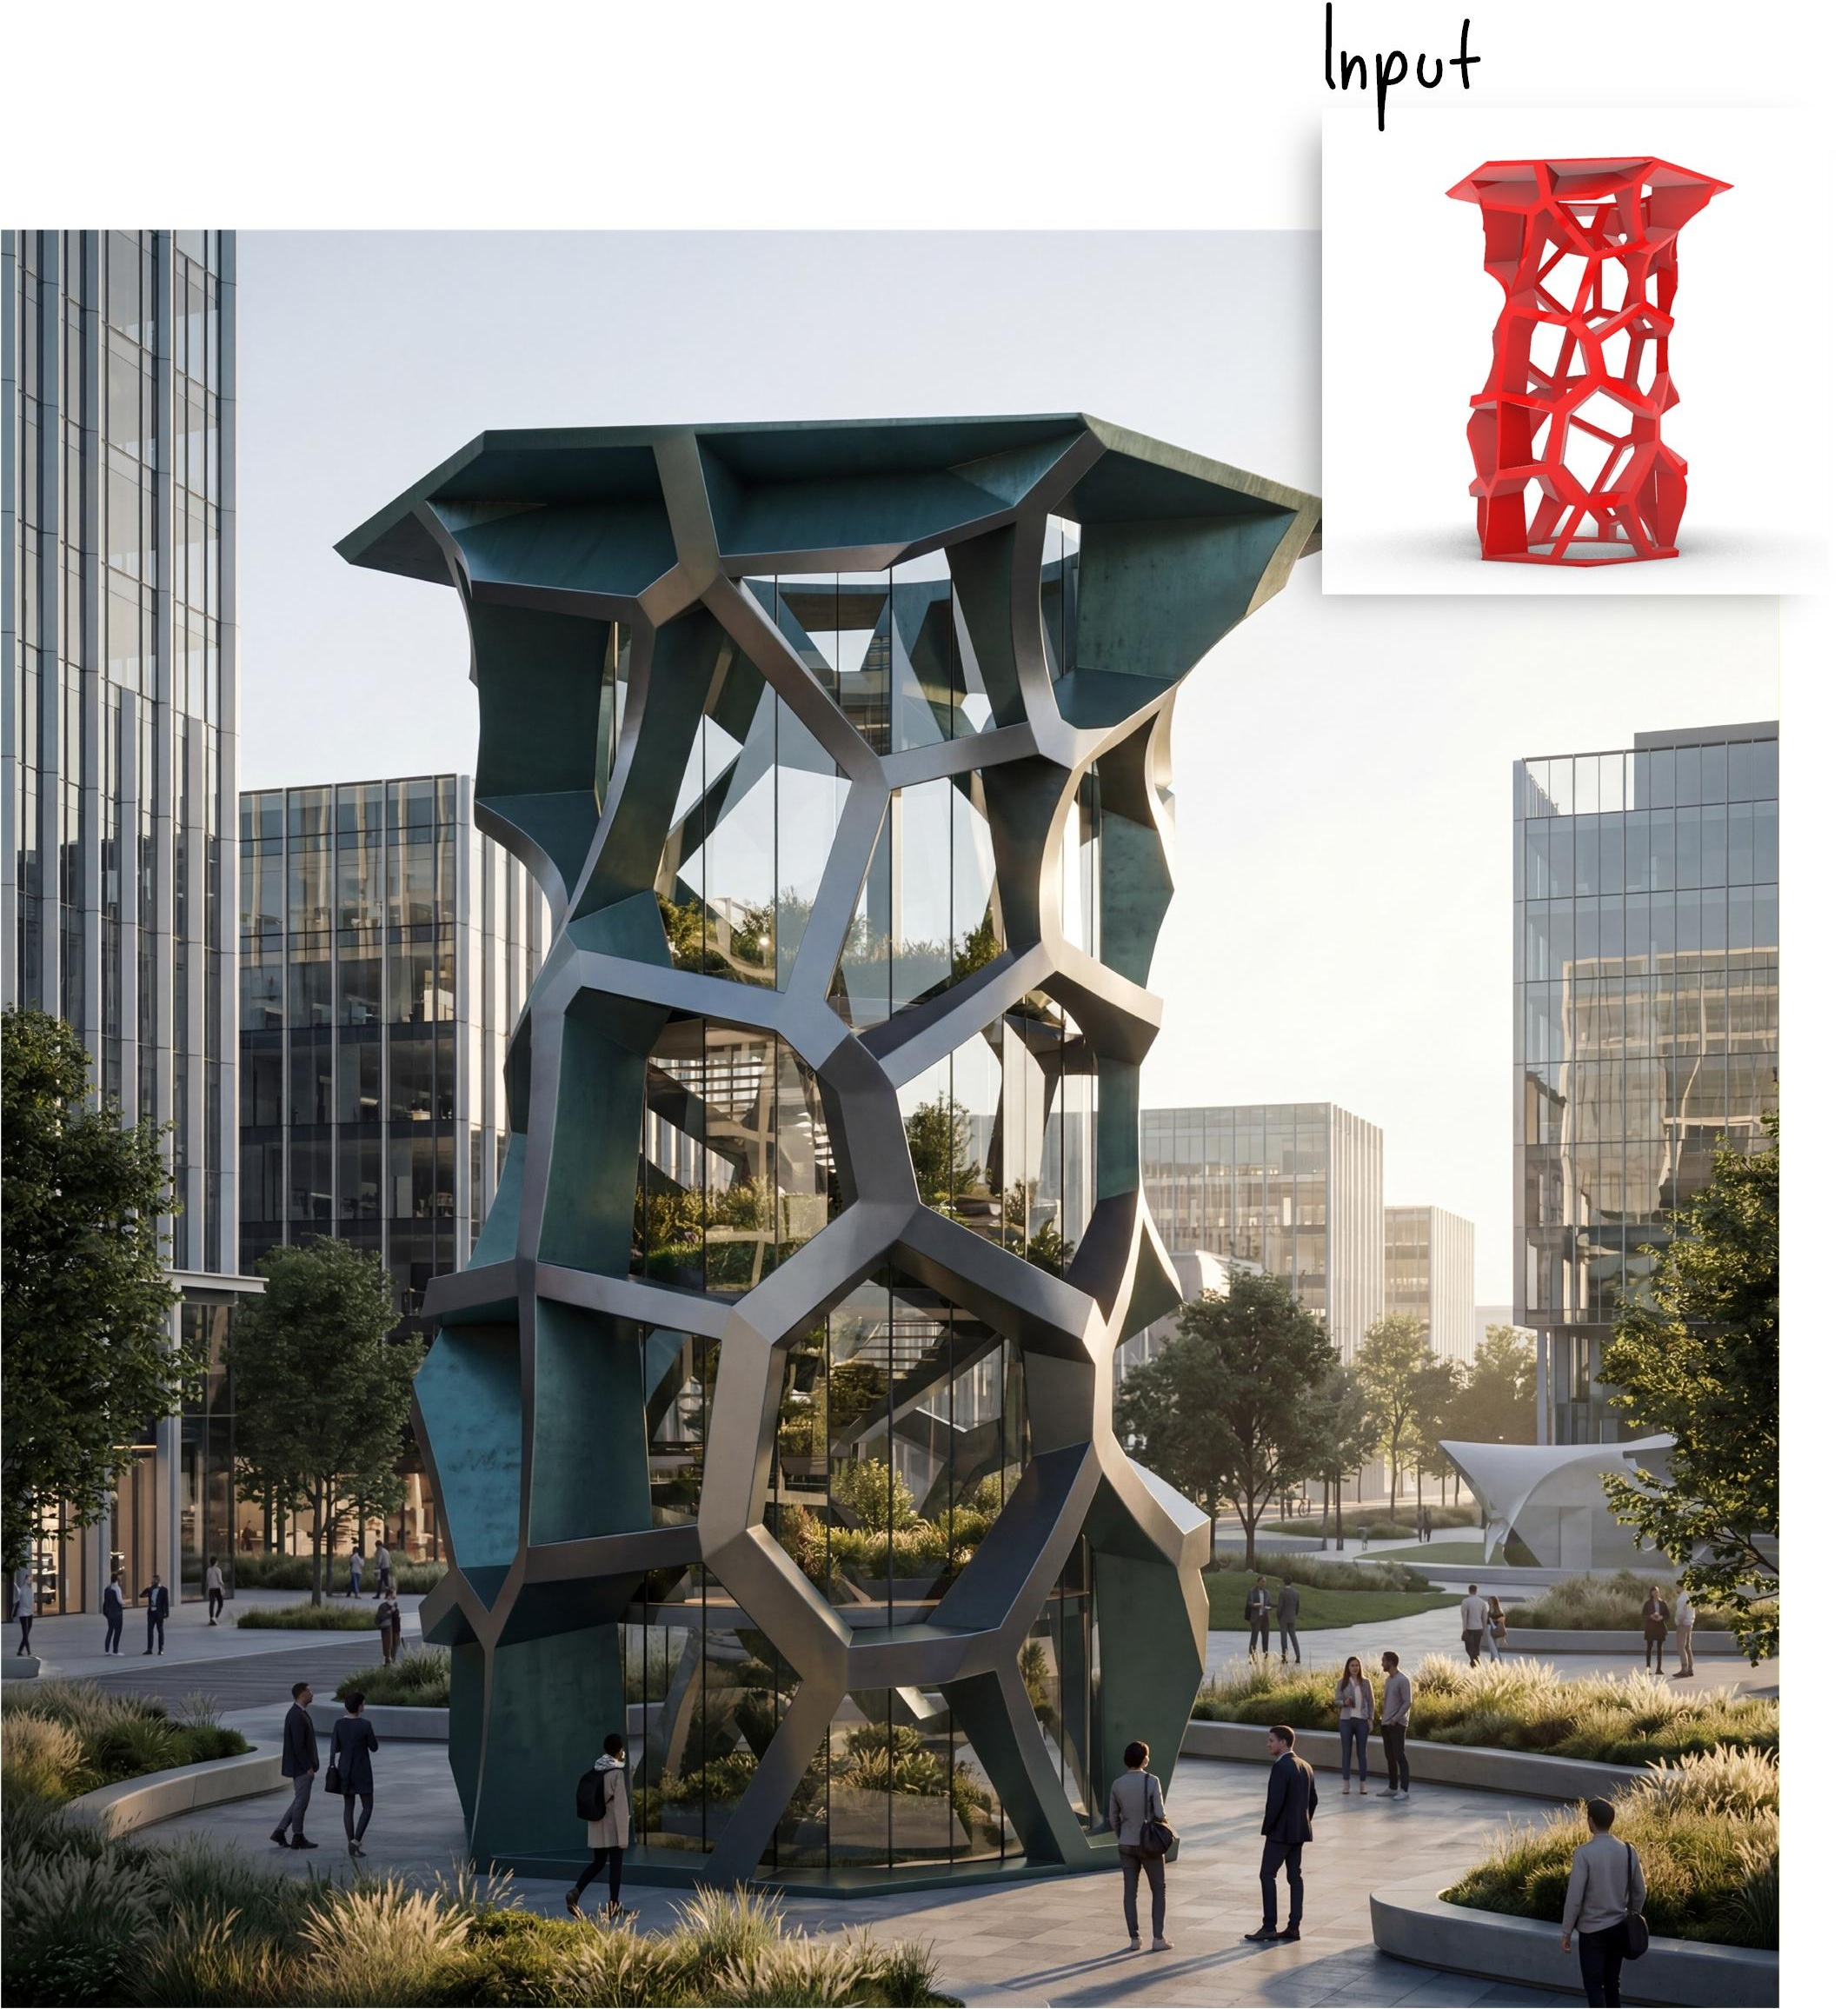
\includegraphics[width=\linewidth]{../resources/practica7/diffusion-images/building_edited.jpg}
  \caption{Torre paramétrica con celosía celular.}
\end{subfigure}\hfill
\begin{subfigure}[t]{0.31\linewidth}
  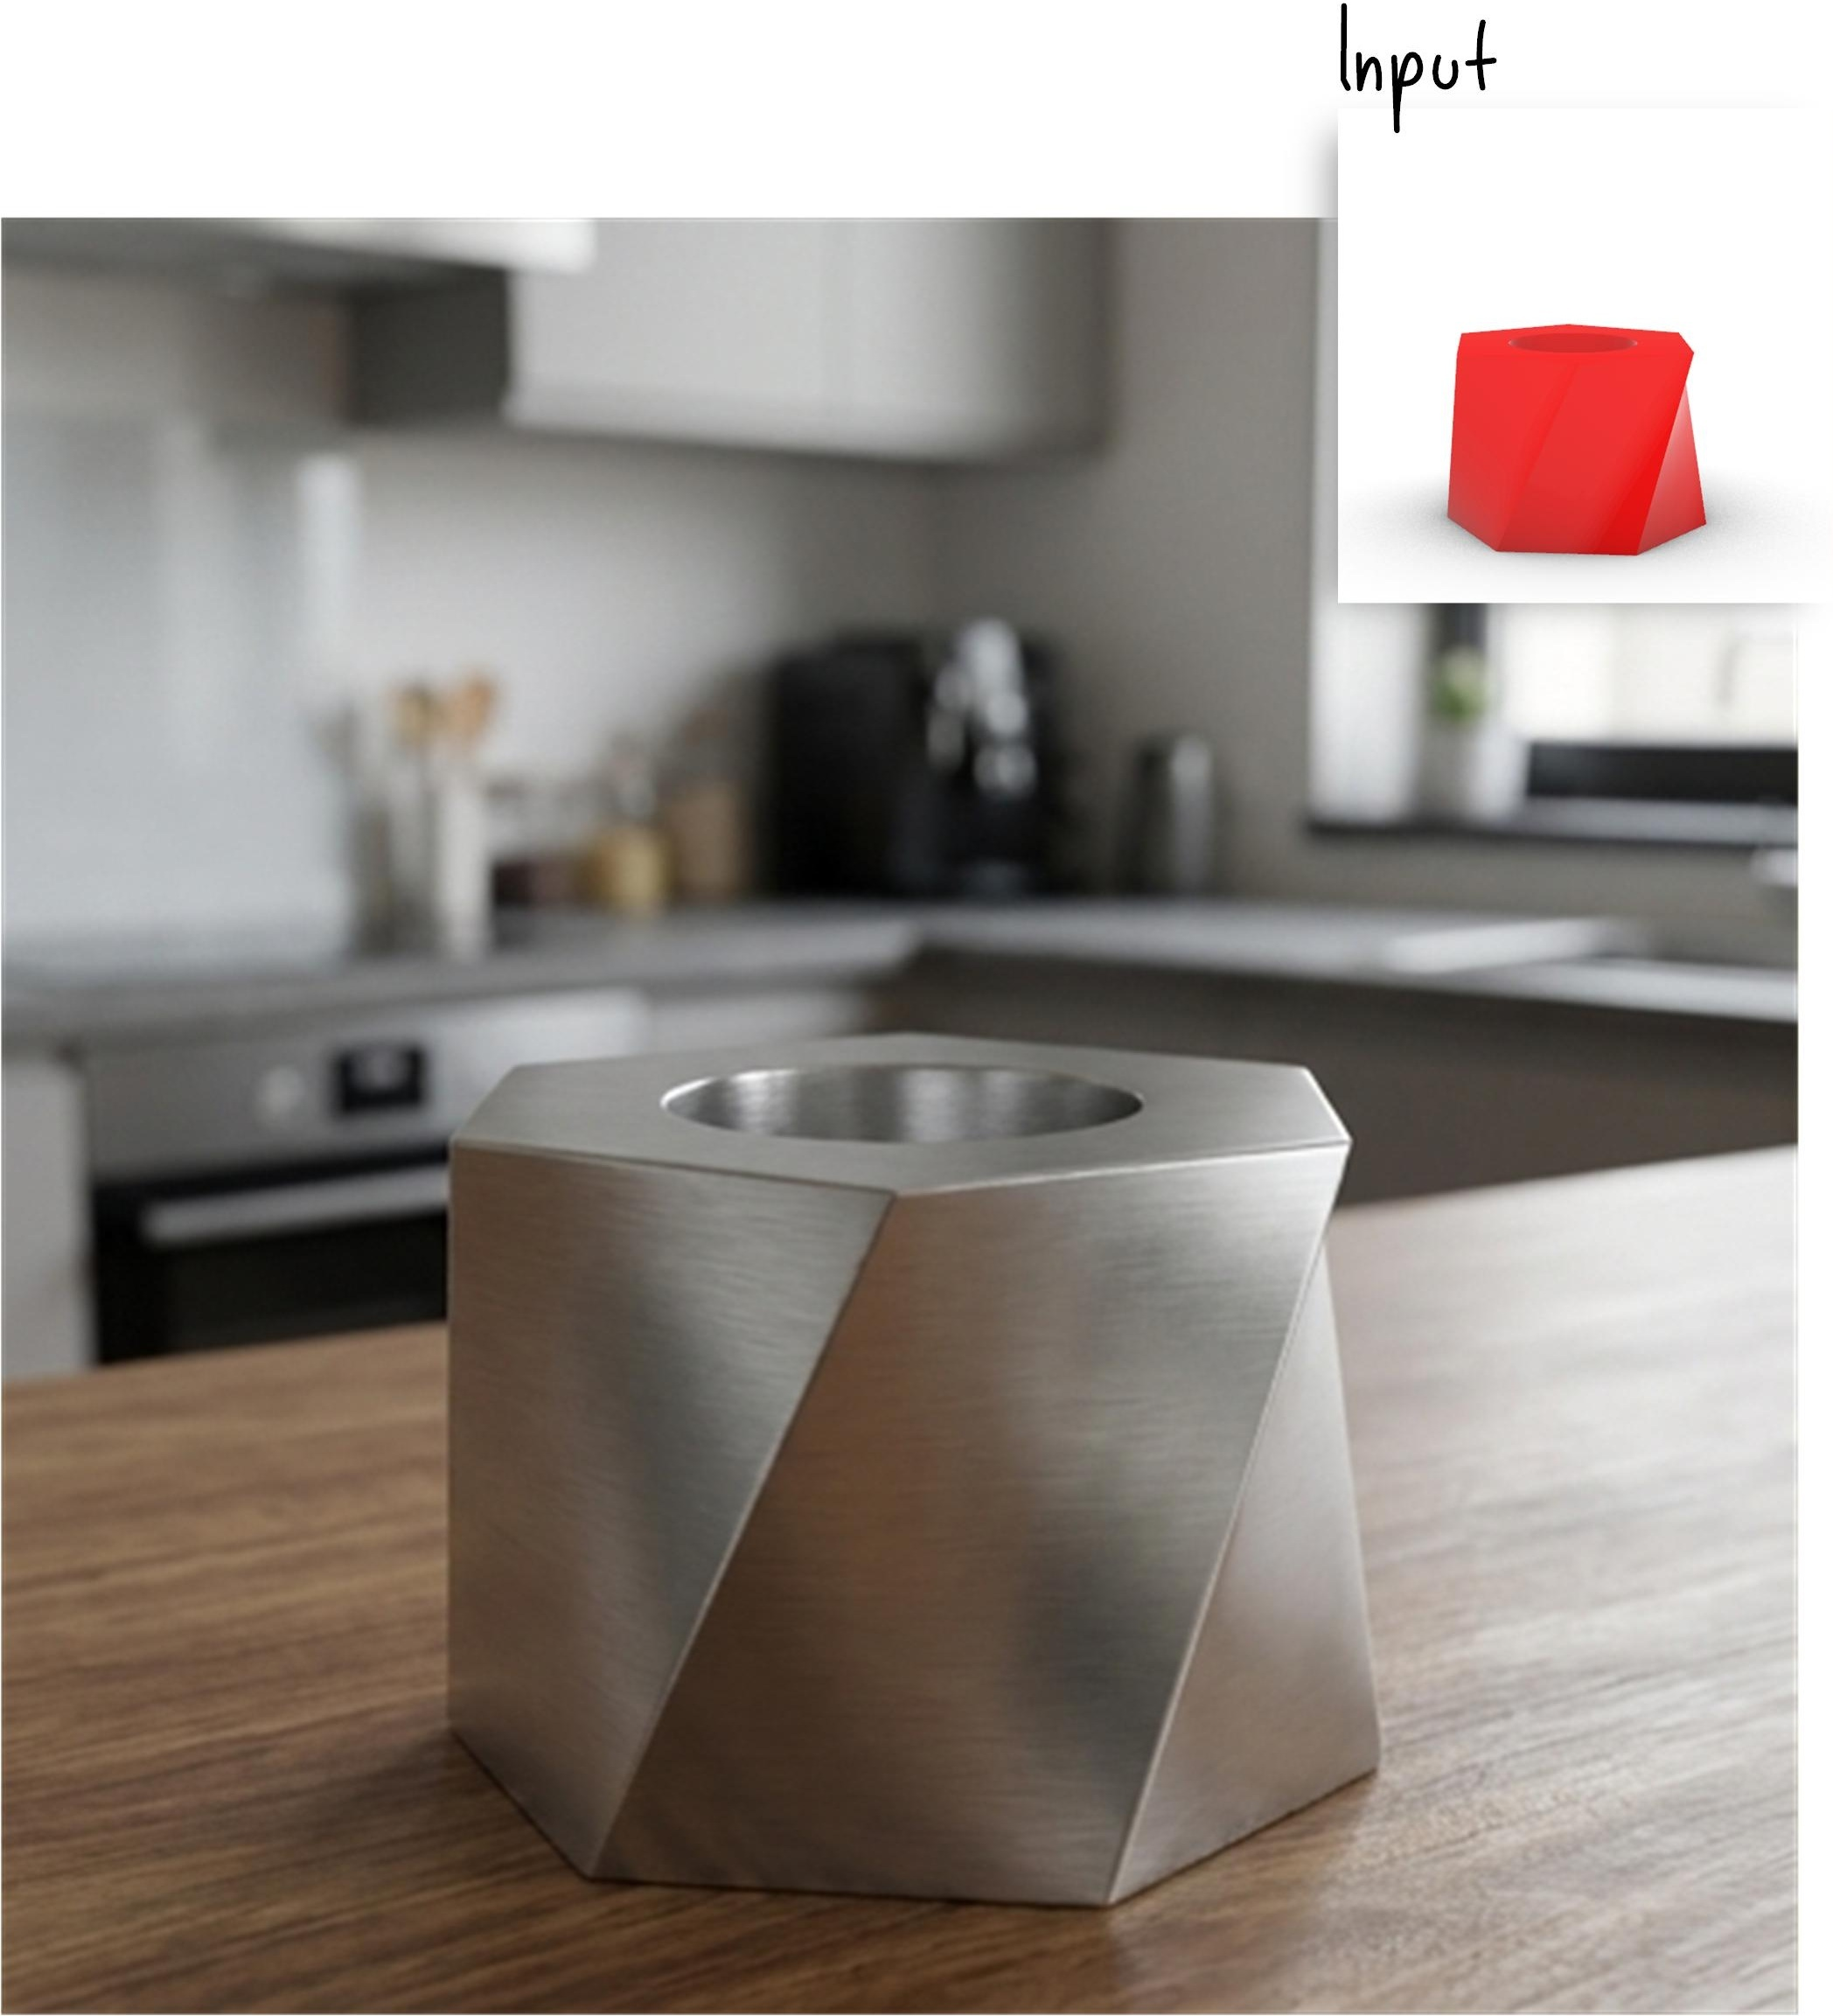
\includegraphics[width=\linewidth]{../resources/practica7/diffusion-images/teacup_edited.jpg}
  \caption{Taza metálica sobre una mesa.}
\end{subfigure}\hfill
\begin{subfigure}[t]{0.31\linewidth}
  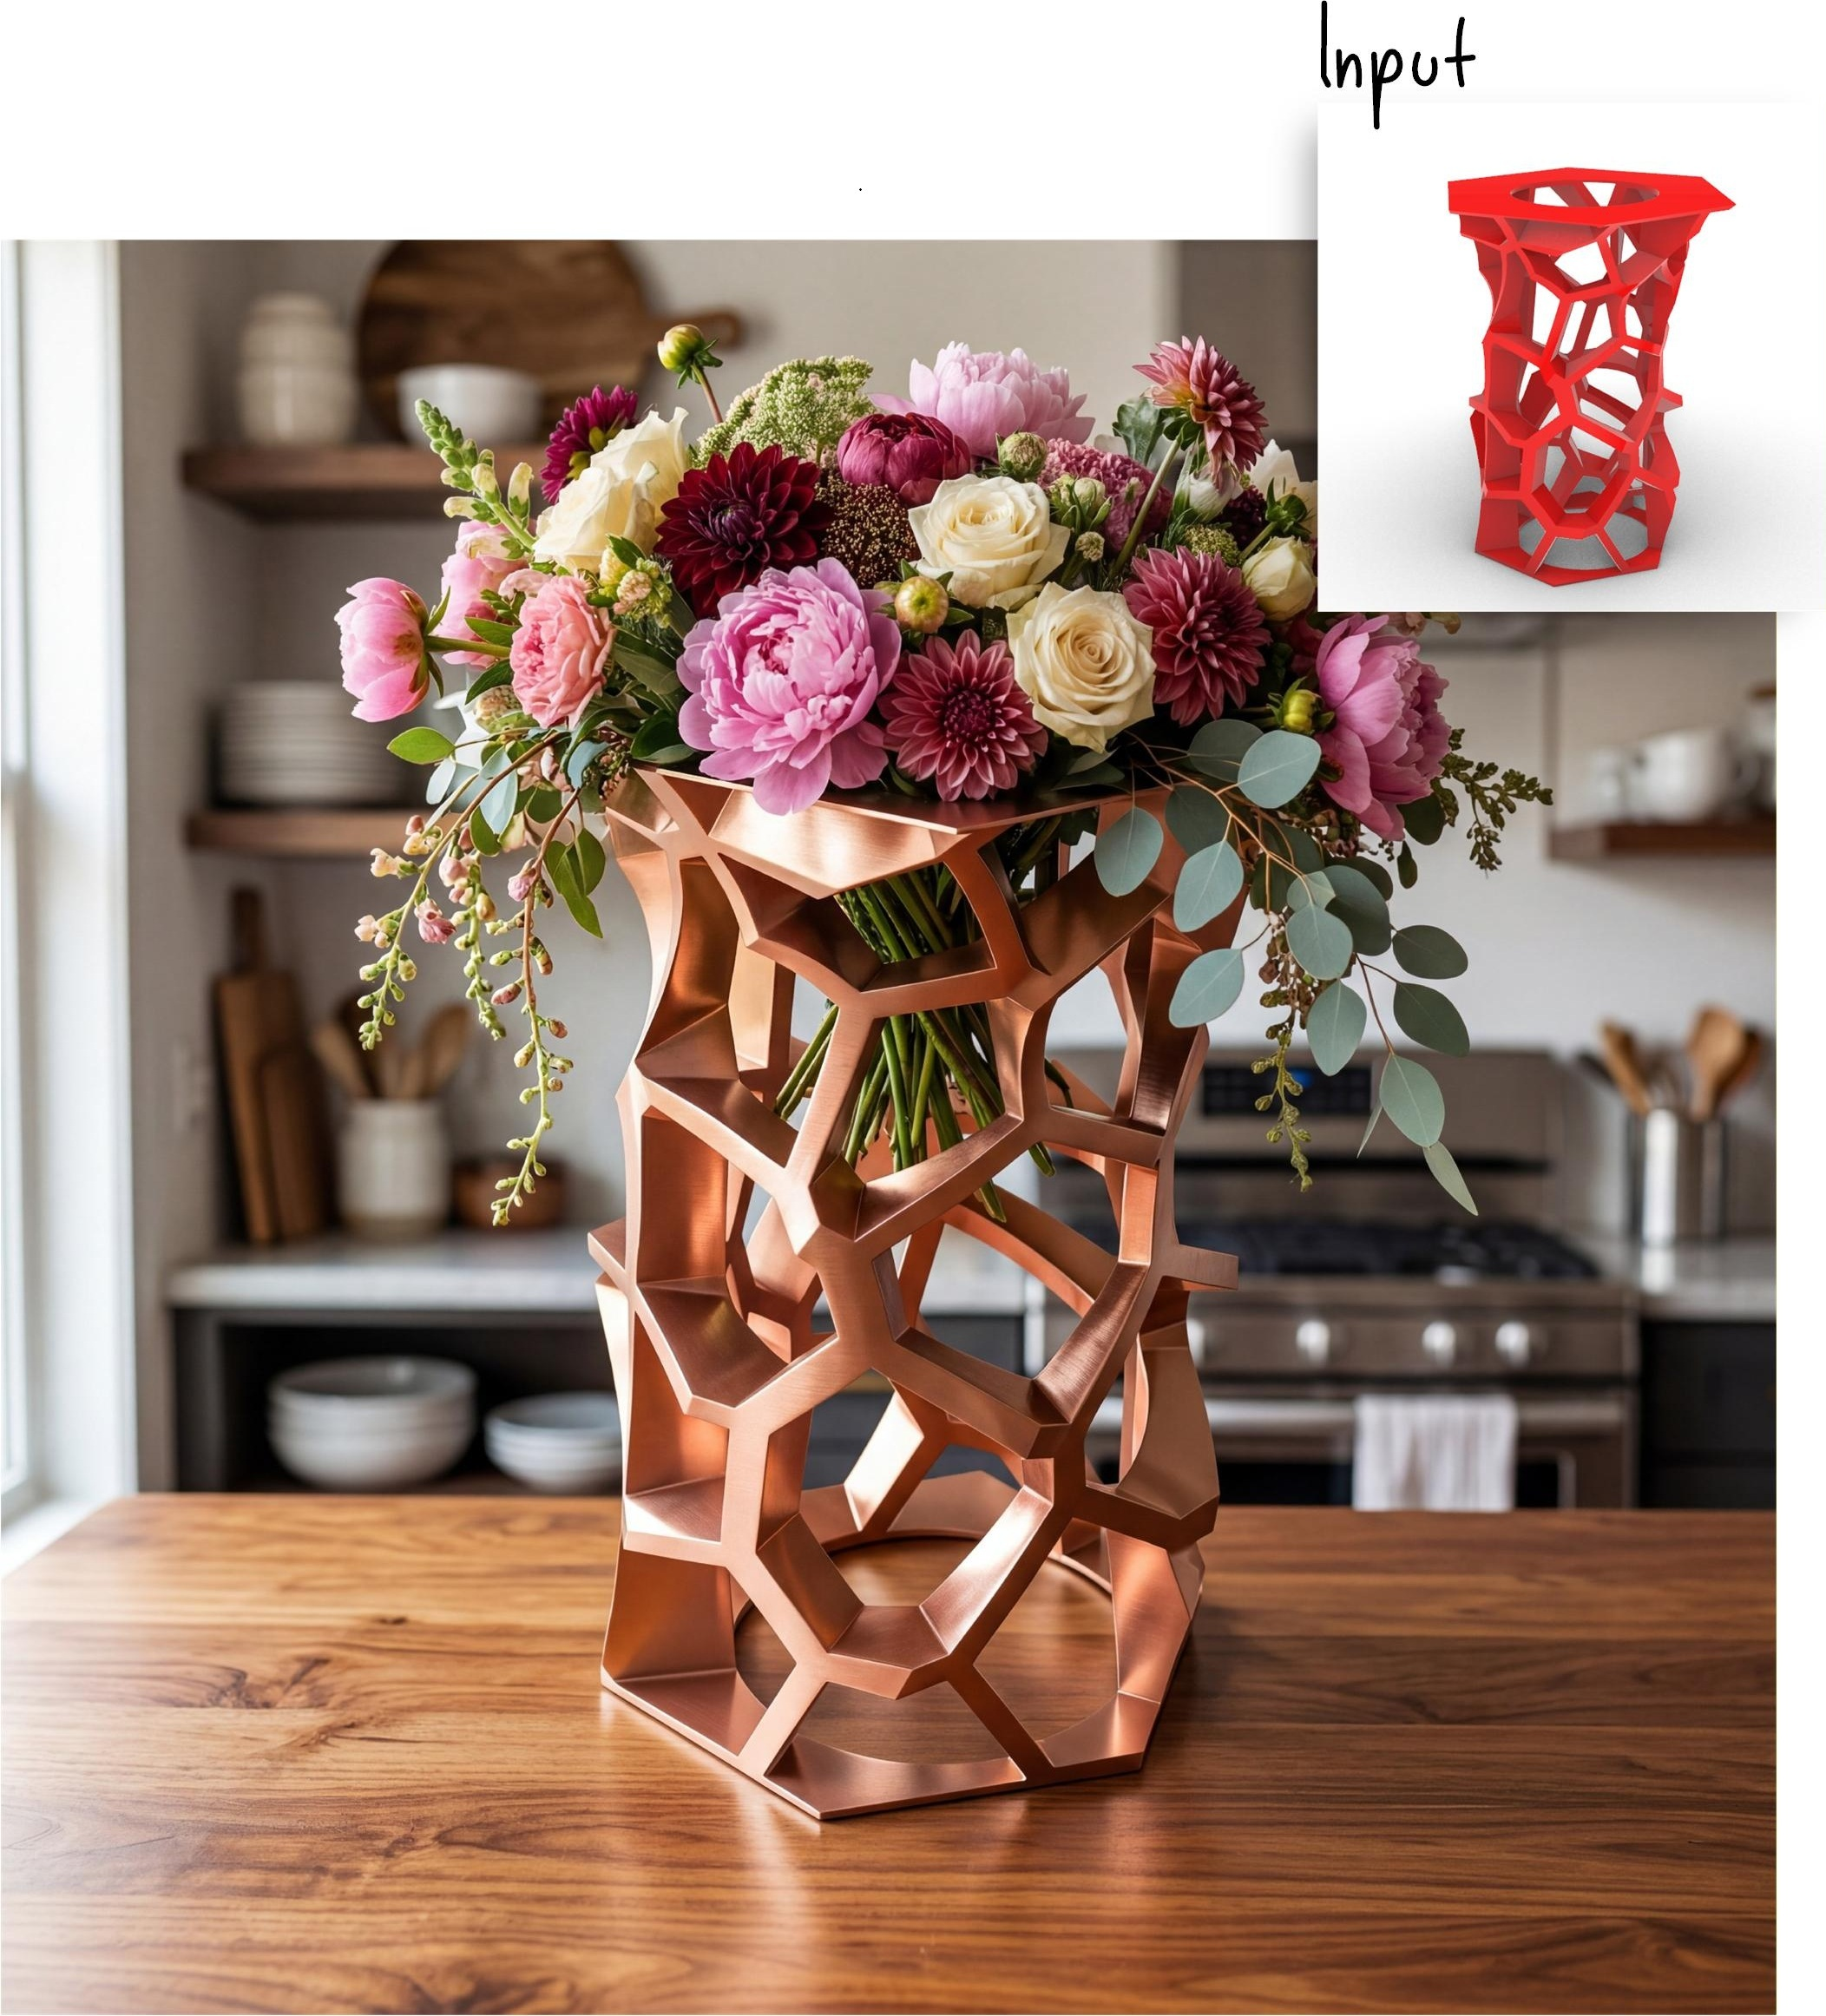
\includegraphics[width=\linewidth]{../resources/practica7/diffusion-images/vase_flowers_edited.jpg}
  \caption{Vasija decorativa con flores.}
\end{subfigure}
\caption{Ejemplos de imágenes generadas a partir de geometrías de la práctica y refinadas mediante \emph{prompts}.}\label{fig-diffusion-examples}
\end{figure}

\subsection{Cómo usar Rhino Banana}
\label{como-usar-rhino-banana}

Para comenzar a generar imágenes, abre \textbf{\emph{RhinoBanana}} desde la línea de comandos de \emph{Rhino} escribiendo \texttt{RhinoBanana} y pulsando Enter. Se abrirá una ventana como la que se muestra en la Figura~\ref{fig-rhino-banana}.

\begin{figure}[H]
\PracticeCenteredImage[width=0.52\textwidth,height=0.46\textheight,keepaspectratio]{../resources/practica7/images/rhino_banana.png}
\caption{Interfaz de RhinoBanana.}\label{fig-rhino-banana}
\end{figure}

En esta interfaz podrás:

\begin{itemize}
\tightlist
\item seleccionar la vista que se utilizará como referencia;
\item elegir la proporción de la imagen final;
\item escoger el modelo de difusión;
\item escribir o refinar el \emph{prompt}.
\end{itemize}

Además, la herramienta incluye un \textbf{\emph{Prompt agent}} que, a partir de una descripción breve, puede ayudarte a generar un \emph{prompt} más largo y elaborado, o a ajustar los parámetros del proceso de generación para conseguir un resultado más cercano a lo que buscas.

\begin{PracticeNoteBox}{Recomendación}
Empieza con un \emph{prompt} simple y claro. Si el resultado no se parece a lo que buscas, añade después detalles sobre material, iluminación, contexto o estilo. Suele funcionar mejor que escribir desde el principio un texto muy largo sin saber qué parte está influyendo en la imagen.
\end{PracticeNoteBox}

\section{Qué debes entregar}
\label{que-debes-entregar}

\textbf{Sólo debe realizar la entrega un miembro del grupo.} Sube a Moodle un fichero comprimido \texttt{practica7.zip} que contenga:

\begin{itemize}
\tightlist
\item \texttt{taza.obj}, con la geometría de la taza modelada en \emph{Grasshopper};
\item \texttt{vasija.obj}, con la geometría de la vasija modelada en \emph{Grasshopper};
\item \texttt{imagen.jpeg}, una imagen generada con un modelo de difusión a partir de una vista de la vasija.
\end{itemize}

\begin{PracticeImportantBox}{Exportar la geometría}
Para exportar la geometría de la taza y la vasija, selecciona cada una de ellas en \emph{Rhino} y ve a \texttt{Archivo > Exportar selección}. Elige el formato \textbf{Wavefront OBJ} y guarda el fichero con el nombre correspondiente (\texttt{taza.obj} o \texttt{vasija.obj}).
\end{PracticeImportantBox}

\end{document}
